\documentclass{article}\usepackage[]{graphicx}\usepackage[]{color}
%% maxwidth is the original width if it is less than linewidth
%% otherwise use linewidth (to make sure the graphics do not exceed the margin)
\makeatletter
\def\maxwidth{ %
  \ifdim\Gin@nat@width>\linewidth
    \linewidth
  \else
    \Gin@nat@width
  \fi
}
\makeatother

\definecolor{fgcolor}{rgb}{0.345, 0.345, 0.345}
\newcommand{\hlnum}[1]{\textcolor[rgb]{0.686,0.059,0.569}{#1}}%
\newcommand{\hlstr}[1]{\textcolor[rgb]{0.192,0.494,0.8}{#1}}%
\newcommand{\hlcom}[1]{\textcolor[rgb]{0.678,0.584,0.686}{\textit{#1}}}%
\newcommand{\hlopt}[1]{\textcolor[rgb]{0,0,0}{#1}}%
\newcommand{\hlstd}[1]{\textcolor[rgb]{0.345,0.345,0.345}{#1}}%
\newcommand{\hlkwa}[1]{\textcolor[rgb]{0.161,0.373,0.58}{\textbf{#1}}}%
\newcommand{\hlkwb}[1]{\textcolor[rgb]{0.69,0.353,0.396}{#1}}%
\newcommand{\hlkwc}[1]{\textcolor[rgb]{0.333,0.667,0.333}{#1}}%
\newcommand{\hlkwd}[1]{\textcolor[rgb]{0.737,0.353,0.396}{\textbf{#1}}}%

\usepackage{framed}
\makeatletter
\newenvironment{kframe}{%
 \def\at@end@of@kframe{}%
 \ifinner\ifhmode%
  \def\at@end@of@kframe{\end{minipage}}%
  \begin{minipage}{\columnwidth}%
 \fi\fi%
 \def\FrameCommand##1{\hskip\@totalleftmargin \hskip-\fboxsep
 \colorbox{shadecolor}{##1}\hskip-\fboxsep
     % There is no \\@totalrightmargin, so:
     \hskip-\linewidth \hskip-\@totalleftmargin \hskip\columnwidth}%
 \MakeFramed {\advance\hsize-\width
   \@totalleftmargin\z@ \linewidth\hsize
   \@setminipage}}%
 {\par\unskip\endMakeFramed%
 \at@end@of@kframe}
\makeatother

\definecolor{shadecolor}{rgb}{.97, .97, .97}
\definecolor{messagecolor}{rgb}{0, 0, 0}
\definecolor{warningcolor}{rgb}{1, 0, 1}
\definecolor{errorcolor}{rgb}{1, 0, 0}
\newenvironment{knitrout}{}{} % an empty environment to be redefined in TeX

\usepackage{alltt}
\usepackage{amscd, amssymb, amsmath, verbatim, setspace}
\usepackage[left=1.0in, right=1.0in, top=1.0in, bottom=1.0in]{geometry}
\usepackage{mathrsfs}
\usepackage{listings}


\IfFileExists{upquote.sty}{\usepackage{upquote}}{}
\begin{document}

\begin{flushright}
  Arif Ali\\
  ANLY-511 Prob. Modeling \& Stat. Computing\\
	Nov 7, 2015\\
\end{flushright}

\begin{center}
  \LARGE\textbf{Homework \#8}
\end{center}
\section*{Problem 57}
\begin{knitrout}
\definecolor{shadecolor}{rgb}{1, 1, 1}\color{fgcolor}\begin{kframe}
\begin{verbatim}
load("~/Dropbox/School/Georgetown/Analytics 511 Fall 2015/hw8.RData")
setwd("~/Dropbox/School/Georgetown/Analytics 511 Fall 2015/")
GS2002 = read.csv("ChiharaHesterberg/GSS2002.csv")
X2GE = chisq.test(table(GS2002[,c("Gender", "Education")]))
X2GE$p.value
## [1] 0.08075942
X2GE$parameter == prod(dim(table(GS2002[,c("Gender", "Education")]))-1)
##   df 
## TRUE
X2HP = chisq.test(table(GS2002[,c("Happy", "PolParty")]))
\end{verbatim}


{\ttfamily\noindent\color{warningcolor}{\#\# Warning in chisq.test(table(GS2002[, c("{}Happy"{}, "{}PolParty"{})])): Chi-squared approximation may be incorrect}}\begin{verbatim}
X2HP$p.value
## [1] 0.0005633274
#X2HP$stdres
#X2HP$residuals
X2HP$parameter == prod(dim(table(GS2002[,c("Happy", "PolParty")]))-1)
##   df 
## TRUE
\end{verbatim}
\end{kframe}
\end{knitrout}
Please note, in order to calculate the degrees of freedom, we do the following : $(r-1)*(c-1)$. In my R code, I checked to make sure that this formula held.

Given the P-value of the Chi-square test with 4 degrees of freedom between Gender and Education is greater than 0.05, so the null hypothesis that the attributes are independent should not be rejected. 

The P-value of the Chi-square test between Happiness and Political Party is significiantly less than 0.05 with 14 degrees of freedom, so the null hypothesis of indepedence is in rejection region. From the standard residuals, it seems like the Republican categories (Near Rep, Not Str Rep, and Strong Rep) are significiantly larger compared to the other categories with respect to Very Happy. There is a warning possibly becuase the data is very sparse.
\section*{Problem 58}
\subsection*{Gender and education}
Since Gender has one of two possiblities, this something that needs to be determined ahead of time for a sample, it would seem more appropriate that indepedence of attributes should be tested instead of homogeneity.
\subsection*{Race and education}
Multiple possiblities for both race and education, so sampling would have to be done by race, thus homogeneity of distributions seems more appropriate.
\subsection*{Happiness and political party}
Homogeneity, you want to know the political party of the people sampled.
\subsection*{Gender and views of death penalty}
Independence, you can collect gender imformation during a sample.
\subsection*{Views of gun laws and race}
Homogeneity, because sampling would be done by targeting race.
\section*{Problem 59}
\begin{knitrout}
\definecolor{shadecolor}{rgb}{1, 1, 1}\color{fgcolor}\begin{kframe}
\begin{verbatim}
load("~/Dropbox/School/Georgetown/Analytics 511 Fall 2015/hw8.RData")
mytable = table(Problem59)
expected = outer(rowSums(mytable), colSums(mytable))/sum(mytable)
unique(expected)
##   A B C D E F G H J K
## 1 2 2 2 2 2 2 2 2 2 2
myX2 <- function(table){sum((table - expected)^2/expected)}
X2 <- myX2(mytable)

X2permuted = function(dummy){
  n <- nrow(Problem59)
  permtable <- table(Problem59$X,Problem59$Y[sample(n,n,replace = F)])
   return(myX2(permtable))
  }
z <- replicate(10000,X2permuted(0))
hist(z)
abline(v = X2, col = 2, lwd = 2)
\end{verbatim}
\end{kframe}
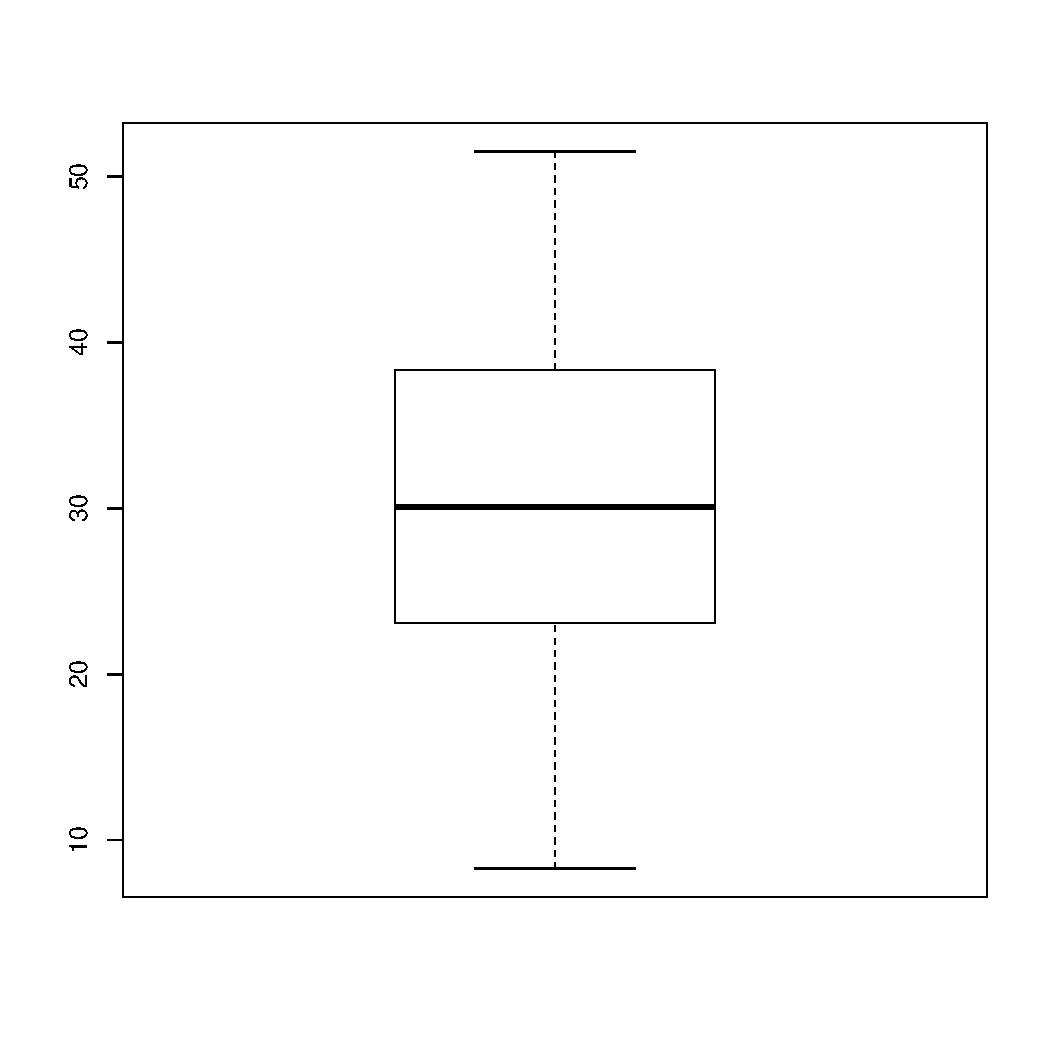
\includegraphics[width=0.33\linewidth]{figure/unnamed-chunk-3-1} 
\begin{kframe}\begin{verbatim}
mean(z > X2)
## [1] 0.7583
mean(z)
## [1] 81.2837
\end{verbatim}
\end{kframe}
\end{knitrout}
The expected value of each cell is small (less than 5); therefore applying a Chi Square test is not usable because you cannot make smooth approximation. Generally Chi-Square tests should have expected values of greater than 5.
\section*{Problem 60}
\subsection*{Part A}
\begin{knitrout}
\definecolor{shadecolor}{rgb}{1, 1, 1}\color{fgcolor}\begin{kframe}
\begin{verbatim}
boxplot(Bangladesh$Arsenic)
hist(Bangladesh$Arsenic)
mean(Bangladesh$Arsenic)
## [1] 125.3199
sd(Bangladesh$Arsenic)/sqrt(length(Bangladesh$Arsenic))
## [1] 18.10072
\end{verbatim}
\end{kframe}
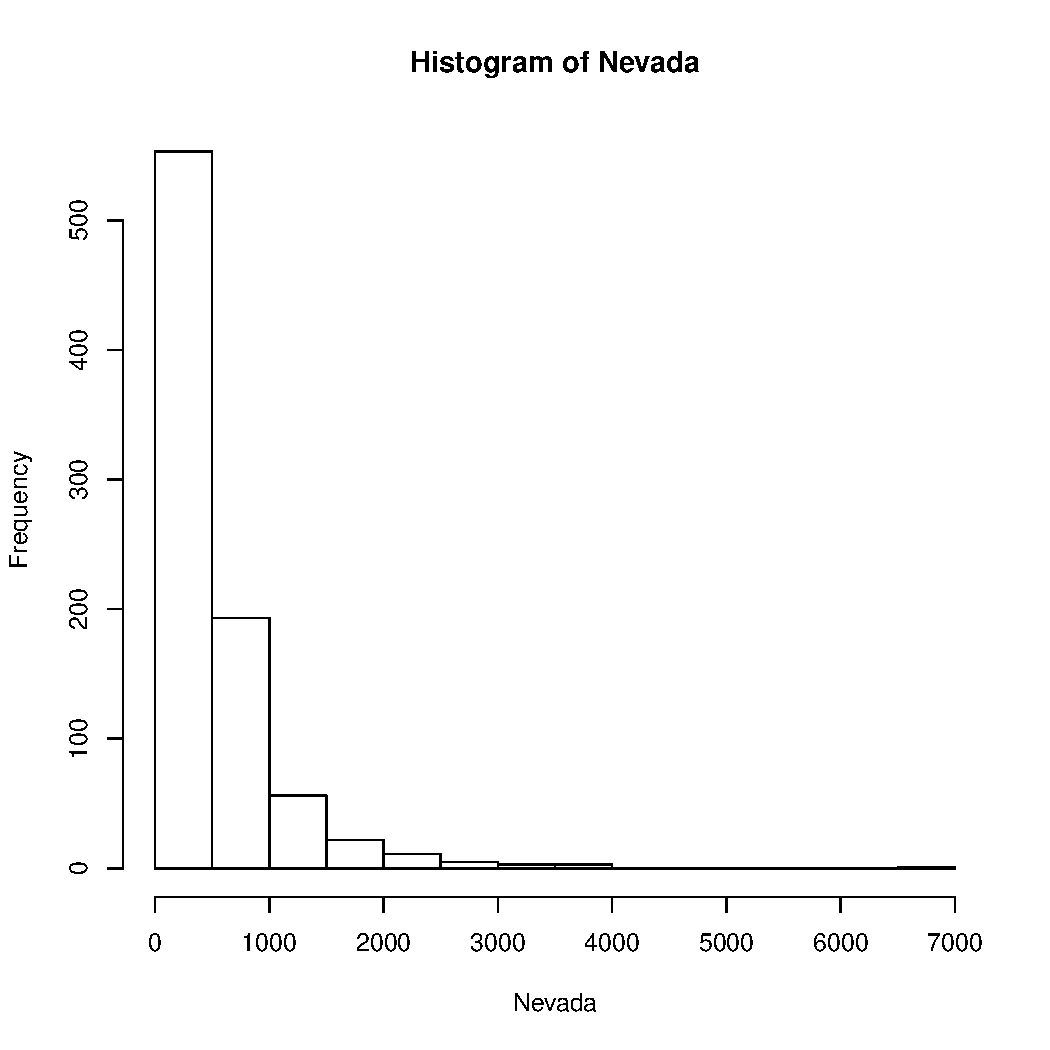
\includegraphics[width=0.33\linewidth]{figure/unnamed-chunk-4-1} 
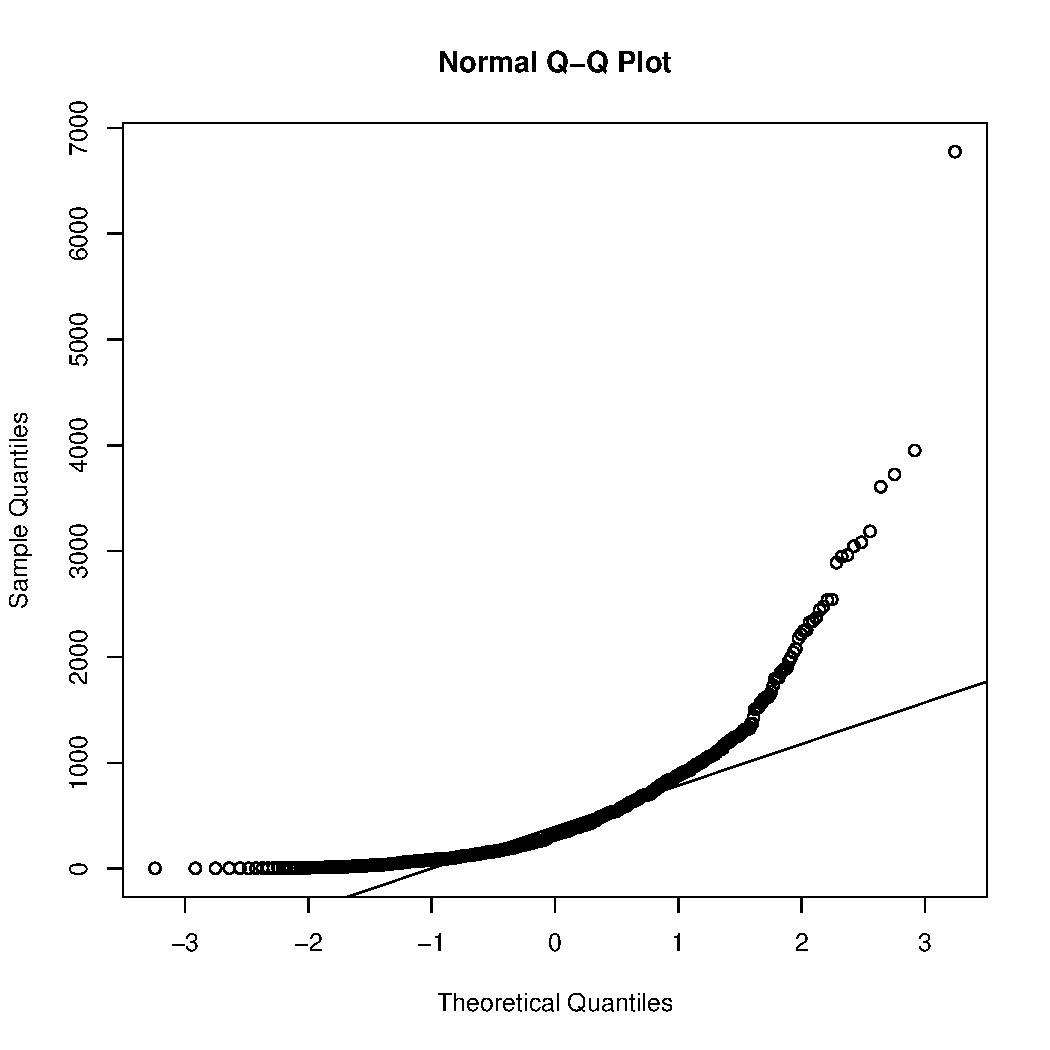
\includegraphics[width=0.33\linewidth]{figure/unnamed-chunk-4-2} 

\end{knitrout}
Based off the boxplot, there seems to be quite a few outliers in the upper bound. Given these are counts of Arsenic, I expected none of the values to be less than zero. The histogram of the arsenic data has characteristics of a poisson distribution.
\subsection*{Part B}
\begin{knitrout}
\definecolor{shadecolor}{rgb}{1, 1, 1}\color{fgcolor}\begin{kframe}
\begin{verbatim}
z <- replicate(100000, mean(sample(Bangladesh$Arsenic,
                                   length(Bangladesh$Arsenic), replace = T)))
mean(z)
## [1] 125.2755
sd(z)
## [1] 18.10015
hist(z, breaks = 50)
boxplot(z)
qqnorm(z)
qqline(z)
\end{verbatim}
\end{kframe}
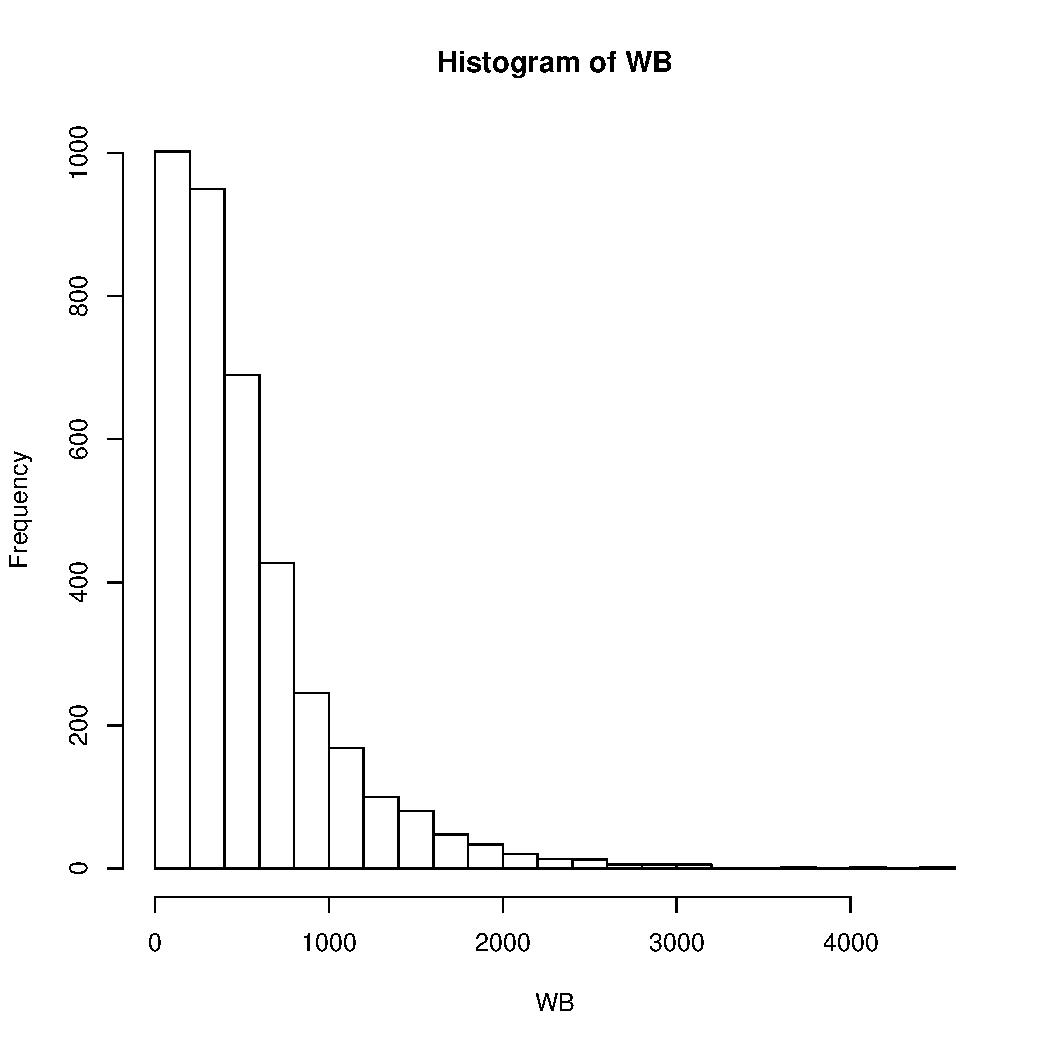
\includegraphics[width=0.33\linewidth]{figure/unnamed-chunk-5-1} 
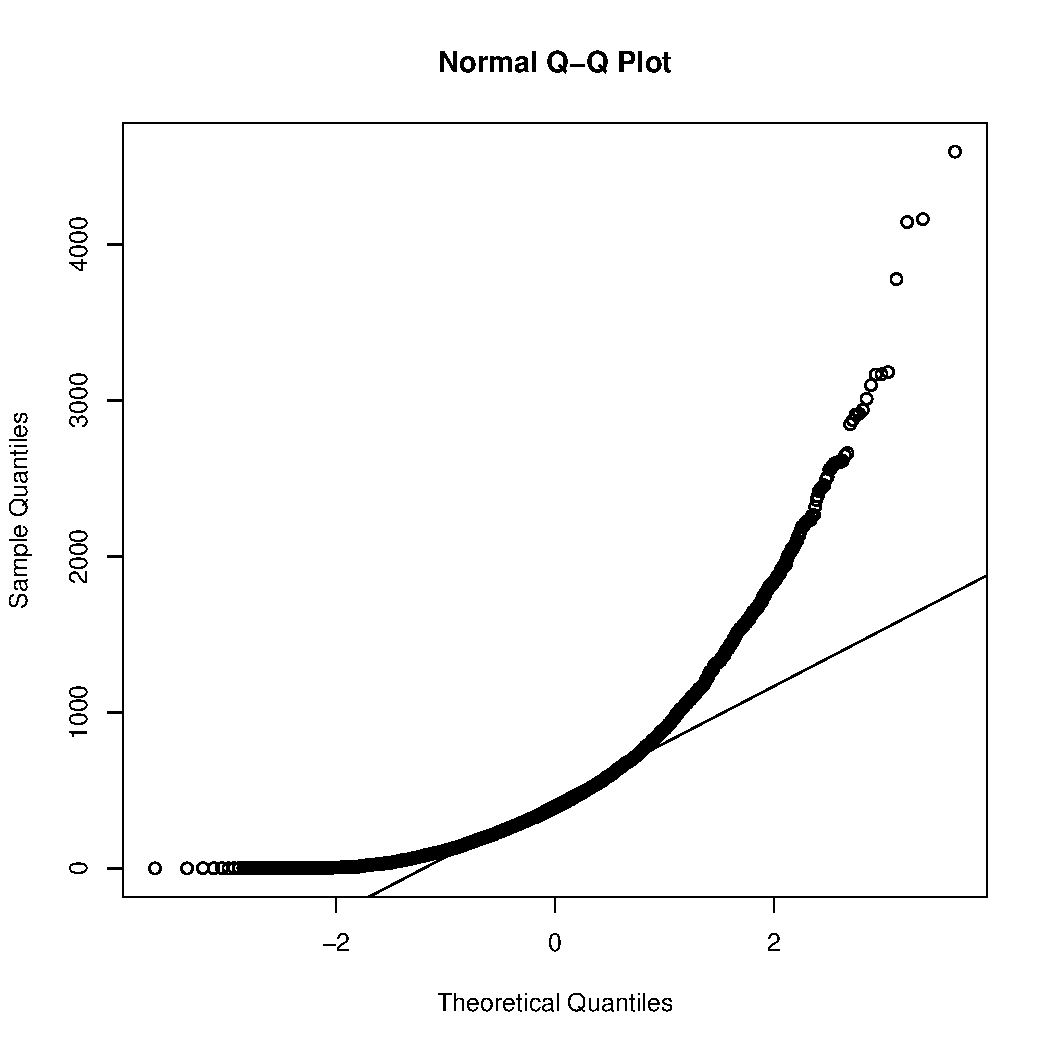
\includegraphics[width=0.33\linewidth]{figure/unnamed-chunk-5-2} 
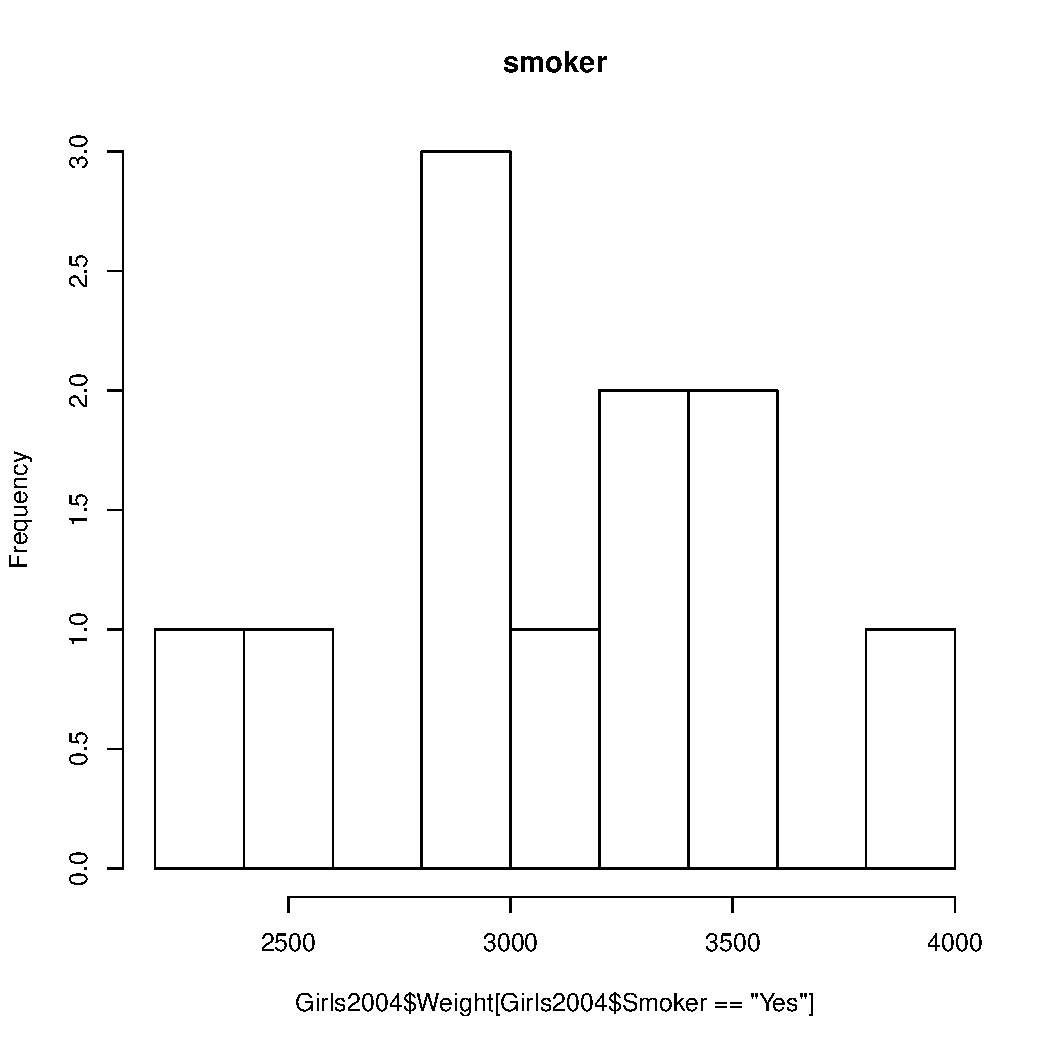
\includegraphics[width=0.33\linewidth]{figure/unnamed-chunk-5-3} 

\end{knitrout}
The histogram looks like a normal distribution, but I ran qqnorm to double check it and with exception to the end points, the bootstrap seems to follow the qqline. Based on the mean and sd, it's a normal distribution with a mean of approximately 125 and a standard deviation of approximately 18. With the boxplot, there are many outliers on the upper and lower bound, but more on the upper bound.
\section*{Problem 61}
\subsection*{Part A}
\begin{knitrout}
\definecolor{shadecolor}{rgb}{1, 1, 1}\color{fgcolor}\begin{kframe}
\begin{verbatim}
Bangladesh_Chlorine = na.omit(Bangladesh$Chlorine)
boxplot(Bangladesh_Chlorine)
hist(Bangladesh_Chlorine)
mean(Bangladesh_Chlorine)
## [1] 78.08401
sd(Bangladesh_Chlorine)/sqrt(length(Bangladesh_Chlorine))
## [1] 12.8051
\end{verbatim}
\end{kframe}
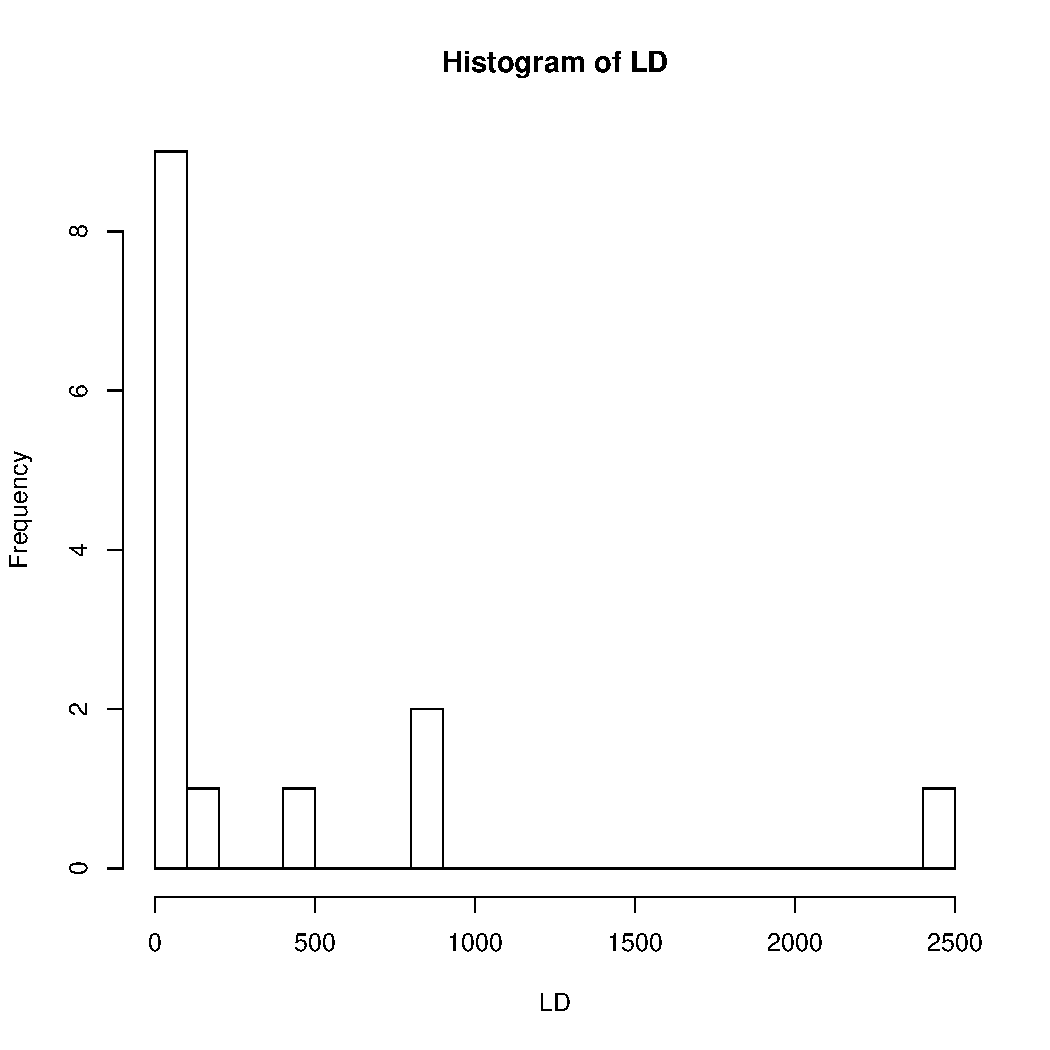
\includegraphics[width=0.33\linewidth]{figure/unnamed-chunk-6-1} 
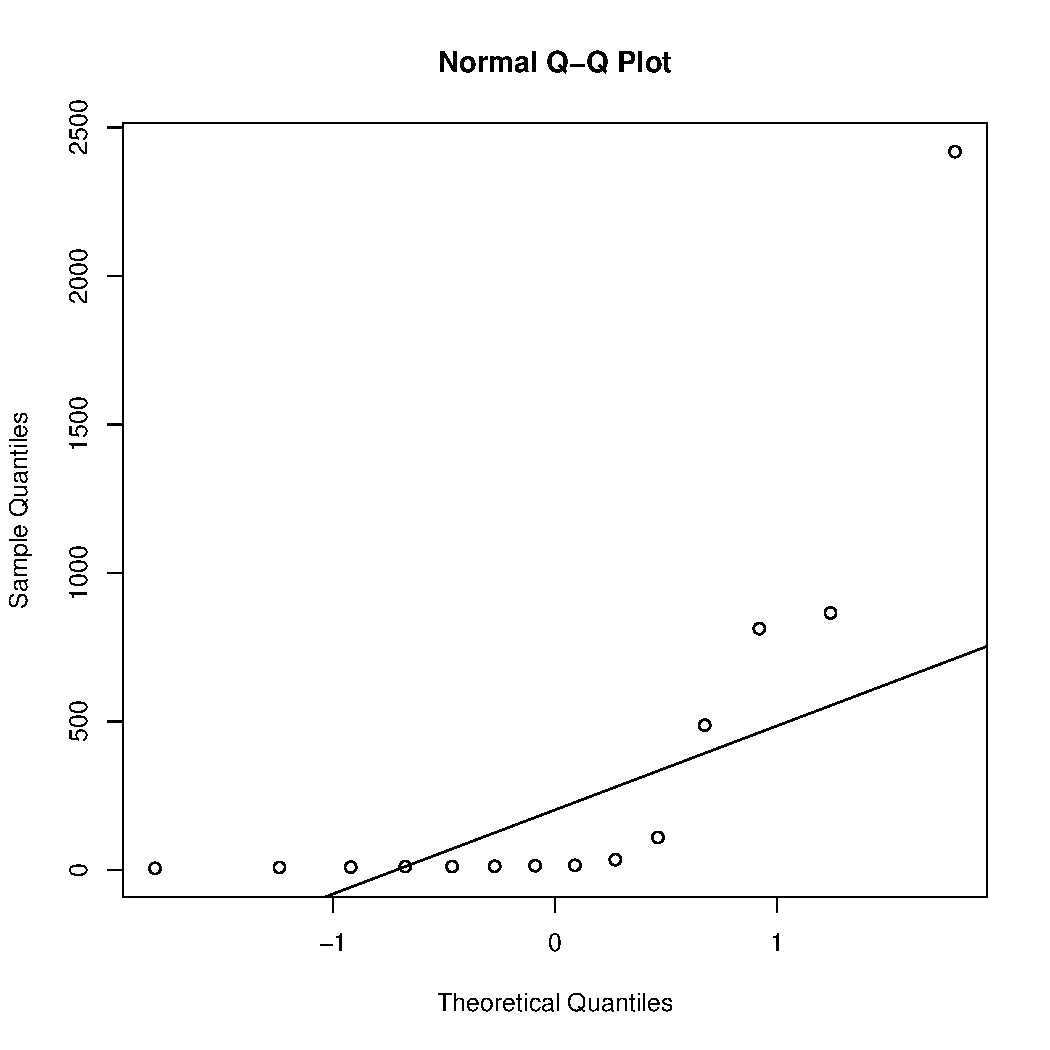
\includegraphics[width=0.33\linewidth]{figure/unnamed-chunk-6-2} 

\end{knitrout}
Much like the Arsenic sample, the outliers are exclusively on the upper bound; however, it is significiantly more spread out, from approximately 100 to over 1500. The Histogram seems like a slightly skewed poisson distribution.
\subsection*{Part B}
\begin{knitrout}
\definecolor{shadecolor}{rgb}{1, 1, 1}\color{fgcolor}\begin{kframe}
\begin{verbatim}
z <- replicate(100000, mean(sample(Bangladesh_Chlorine,
                                   length(Bangladesh_Chlorine), 
                                   replace = T)))
# 90% CI
quantile(z, c(0.05, 0.95), na.rm = T)
##       5%      95% 
##  58.1200 100.0747
\end{verbatim}
\end{kframe}
\end{knitrout}

\section*{Problem 62}
$expected = (2m+20)/4=\frac{1}{2}m+5$
Please note, I plugged the following into wolfram Alpha and got 3.841459 using qchisq(.95,1)
So, $X^{2}=4*\frac{(\frac{1}{2}m-5)^{2}}{\frac{1}{2}m+5}=3.841459$ The m values must be integrers $\therefore 0\leq m\leq 4\;or\;m \geq 18$
 
\section*{Problem 63}
\begin{knitrout}
\definecolor{shadecolor}{rgb}{1, 1, 1}\color{fgcolor}\begin{kframe}
\begin{verbatim}
Problem63 = matrix(c(23, 18,7,13),2)
Problem63.chisq = chisq.test(Problem63)
Problem63.fisher = fisher.test(Problem63)
Problem63.prop = prop.test(Problem63)
Problem63.prop$conf.int
## [1] -0.07716531  0.44920832
## attr(,"conf.level")
## [1] 0.95
\end{verbatim}
\end{kframe}
\end{knitrout}
The difference between the P-values is approximately 0.03, but under both test, the null hypothesis,that the drugs aren't different in terms of healing rate, would not be rejected. The confidence interval is surpisely large. From the odd's ratio, it seems like the odds of being healed to not healed indicates that people do get healed on either drug.
\section*{Problem 64}
\subsection*{Part A}
\begin{knitrout}
\definecolor{shadecolor}{rgb}{1, 1, 1}\color{fgcolor}\begin{kframe}
\begin{verbatim}
quantile(Bangladesh$Arsenic, c(0.5, .90))
## 50% 90% 
##  22 270
\end{verbatim}
\end{kframe}
\end{knitrout}
\subsection*{Part B}
\begin{knitrout}
\definecolor{shadecolor}{rgb}{1, 1, 1}\color{fgcolor}\begin{kframe}
\begin{verbatim}
z <- replicate(100000, median(sample(Bangladesh$Arsenic,
                                    length(Bangladesh$Arsenic), 
                                    replace = T)))
bias_median = median(Bangladesh$Arsenic) - mean(z)
bias_median
## [1] -1.456376
\end{verbatim}
\end{kframe}
\end{knitrout}

\subsection*{Part C}
\begin{knitrout}
\definecolor{shadecolor}{rgb}{1, 1, 1}\color{fgcolor}\begin{kframe}
\begin{verbatim}
z <- replicate(100000, quantile(sample(Bangladesh$Arsenic,
                                      length(Bangladesh$Arsenic), 
                                      replace = T),0.9))
bias_90percentile = quantile(Bangladesh$Arsenic,0.9) - mean(z)
bias_90percentile
##      90% 
## -3.45719
\end{verbatim}
\end{kframe}
\end{knitrout}

\end{document}
